\sect{5. How to play}

\begin{figure}[H]
\centering
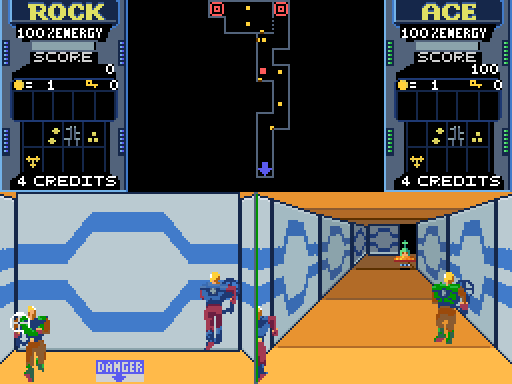
\includegraphics[width=0.48\textwidth]{../img/play_l1.png}\hfill
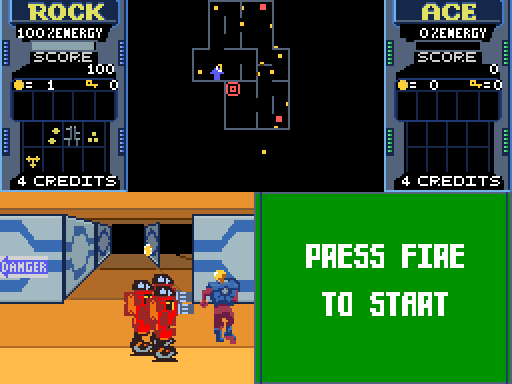
\includegraphics[width=0.48\textwidth]{../img/play_l5.png}
\caption{Left: Rock and Ace in the first level, each in their own view. Right: robots in level 5.}
\end{figure}

Rock (player 1) and Ace (player 2) go through the mazes of the Xybots' city, seen from behind the hero. Each level is a maze full
of robots, coins, keys and energy. \textbf{Find the exit of the level and walk into it.} The level number is shown before it starts
(\texttt{PREPARE TO ENTER LEVEL}).

\begin{itemize}
\item \textbf{Robots.} Shoot them; tougher ones need several hits. Some walk straight into you: the crash takes 25 energy. Robots can
pick up objects and drop them when they are destroyed. Some walls can be shot away too.
\item \textbf{Energy.} You start with 100. It goes down slowly with time, and with every shot or crash that hits you. At 0 the hero
dies and a credit is used (section 8).
\item \textbf{Keys} open the doors marked on the map. Walking into a locked door uses one key and the door disappears.
\item \textbf{Coins} are the money of the shop between levels (section 7).
\item \textbf{Two players.} Player 2 can join while the game goes on by pressing fire; the screen of Ace says \texttt{PRESS FIRE TO START}.
It is not possible during the shop, bonus and waiting screens or a Master Xybot fight. From level 6 on, \texttt{SHOTS HURT OTHER PLAYERS}:
take care not to hit your partner. When a player dies, the partner gets their keys.
\item \textbf{After the exit} come a bonus screen (if any), the shop and the \texttt{PREPARE} screen. In a two-player game the first one
out shows \texttt{WAITING...} until the partner arrives, and gets \texttt{BONUS FOR EXITING FIRST}: one coin.
\item \textbf{Points}: every object picked up gives 100 points, every robot destroyed gives points as well.
\end{itemize}

\begin{figure}[H]
\centering
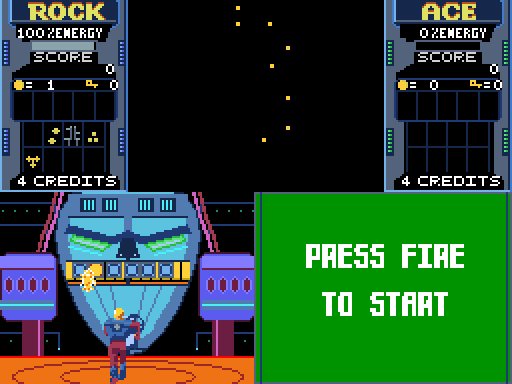
\includegraphics[width=0.48\textwidth]{../img/boss.png}\hfill
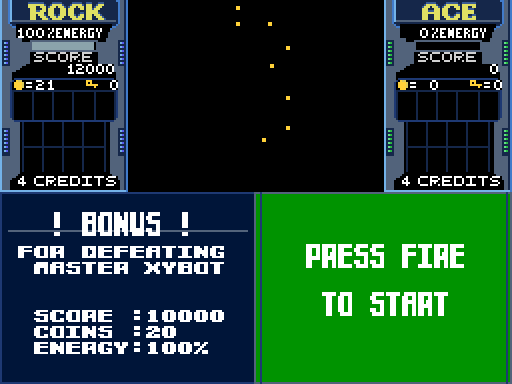
\includegraphics[width=0.48\textwidth]{../img/bonus_boss.png}
\caption{Left: the Master Xybot. Right: the bonus for defeating him.}
\end{figure}

\textbf{The Master Xybot.} Instead of levels 16, 26 and 36 you fight the Master Xybot in his room (\texttt{PREPARE TO FIGHT MASTER XYBOT};
the \texttt{PREPARE} screen warns you a few levels before). His six parts open and close and fire when they are open; they can only be
hurt while open. Destroy all six: \texttt{! BONUS !} gives 10,000 points, 20 coins and full energy, and the game goes on with the next
level. If every player dies in the fight, the game goes back four levels. After the last level the game starts again from level 1,
with tougher robots.

% ==================================================================
\sect{6. The panel}

Each player has a panel: Rock on the left, Ace on the right. The map is in the middle.

\begin{center}
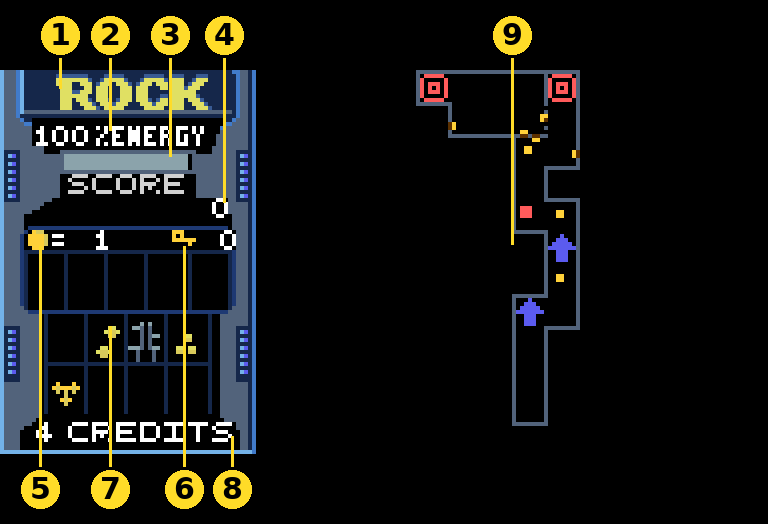
\includegraphics[width=0.85\textwidth]{img/hud.png}
\end{center}

\begin{tabularx}{\textwidth}{@{}clX@{}}
\toprule
\textbf{\tNo} & \textbf{\tElement} & \textbf{\tTellsYou}\\
\midrule
1 & Name & \texttt{ROCK} is player 1, \texttt{ACE} player 2.\\
2 & \texttt{\%ENERGY} & The energy left, from 0 to 100 (125 with \texttt{125\% LIMIT}).\\
3 & Energy bar & The same energy as a bar.\\
4 & \texttt{SCORE} & The points of the player.\\
5 & Coins & The coins the player carries, to spend in the shop.\\
6 & Keys & The keys the player carries.\\
7 & Equipment & An icon for every upgrade or gadget of the shop the player owns.\\
8 & \texttt{CREDITS} & The credits left; both players share them.\\
9 & Map & The part of the maze seen so far: walls, locked doors (dotted), the exits (a square inside a square), the heroes (arrows that
show where they look) and marks for robots and objects. It stays empty in the Master Xybot's room.\\
\bottomrule
\end{tabularx}

% ==================================================================
\sect{7. Objects and the shop}

\textbf{On the floor:} coins (one coin), keys (one key), energy (50 or 100 energy, never above the limit) and the gun power-up: for a
while the shots are stronger and the hero fires two balls at a time, or three when the power-up is taken again.

\begin{figure}[H]
\centering
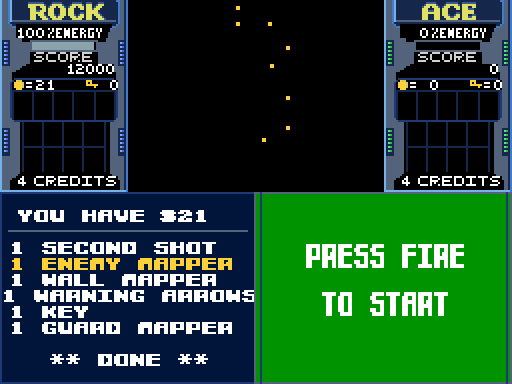
\includegraphics[width=0.55\textwidth]{../img/shop.png}
\caption{The shop: \texttt{YOU HAVE \$21} coins; up and down choose, fire buys.}
\end{figure}

\textbf{The shop} opens after every exit when you have coins. It offers up to six things, with the number of coins each costs in front.
Up and down move the bar, fire buys; \texttt{** DONE **} leaves. The shop closes by itself when your coins run out. Upgrades can be bought
more than once, up to their maximum.

\begin{tabularx}{\textwidth}{@{}lcX@{}}
\toprule
\textbf{Item} & \textbf{Coins} & \textbf{What it does}\\
\midrule
\texttt{MOVE FASTER} & 7 & Walk faster.\\
\texttt{BETTER SHIELD} & 7 & Shots hurt less.\\
\texttt{FAST SHOTS} & 7 & Your shots fly faster.\\
\texttt{SHOT POWER} & 7 & Your shots hurt more.\\
\texttt{ZAP POWER} & 7 & A stronger special attack (it costs more energy too).\\
\texttt{SLOW ENERGY} & 2 & The energy goes down more slowly with time.\\
\texttt{SECOND SHOT} & 1 & Two shots in the air at a time.\\
\texttt{ENEMY MAPPER} & 1 & The robots appear on the map.\\
\texttt{WALL MAPPER} & 1 & The whole maze appears on the map.\\
\texttt{GUARD MAPPER} & 1 & The guard robots appear on the map.\\
\texttt{WARNING ARROWS} & 1 & \texttt{DANGER} signs at the side of the view when a robot can reach you straight.\\
\texttt{50\% ENERGY POD} & 5 & 50 energy.\\
\texttt{SHOTS REPELLED} & 5 & The next five shots that hit you bounce off.\\
\texttt{125\% LIMIT} & 5 & The energy can go up to 125.\\
\texttt{KEY} & 1 & One key.\\
\texttt{GIVE FRIEND} & 1 & Gives one coin to your partner.\\
\bottomrule
\end{tabularx}

\medskip
From level 7 on, the gadgets (second shot, mappers, warning arrows, 125\% limit) wear off: every exit takes one step of each away.

% ==================================================================
\sect{8. Credits, continue and high score}

\begin{itemize}
\item The game starts with \textbf{4 credits}, shared by both players (\texttt{4 CREDITS} in the panel).
\item When a hero dies, one credit is used and the view says \texttt{PRESS FIRE TO CONTINUE}. Fire puts the hero back at the start of
the level with full energy and everything bought kept.
\item The death that uses the \textbf{last credit} ends that player's game: if the score beats the high score, \texttt{NEW HISCORE}
flashes; then \texttt{GAME OVER}. With 4 credits a player can continue three times.
\item The high score starts at 1000 and is shown on the title screen as \texttt{HI:}. It is kept until the MSX is switched off.
\item Joining as player 2 costs no credit.
\end{itemize}

% ==================================================================
\sect{9. Music and voices}

Without a Moonsound you hear the music and sound effects of the original MSX game. With a \textbf{Moonsound}, the music and voices are:

\begin{itemize}
\item a song with voices on the logo screen;
\item the arcade title music with its voices on the title screen;
\item one of four arcade voices, at random, when a game starts;
\item two arcade songs in the levels, one for the odd levels and one for the even ones;
\item the arcade shop music in the shop and on the \texttt{PREPARE} screen;
\item the Master Xybot's music and his voice: when the fight starts, when he is hit, and ``I'll be back'' when he is defeated.
\end{itemize}

With more than 128~KB of Moonsound sample RAM, shots, hits and some pickups, exits and teleports use arcade sounds. Other effects still come from the MSX.

% ==================================================================
\sect{10. Tips}

\begin{itemize}
\item Watch the map: the exits are drawn as a square inside a square. Doors need keys, so pick them up on the way.
\item Some levels hide a \textbf{warp exit}: \texttt{WARP BONUS} takes you straight to level 7 with 25 coins, full energy and 75,000 points.
\item Keep coins for the shop: \texttt{SHOT POWER}, \texttt{BETTER SHIELD} and \texttt{SLOW ENERGY} help in the long run.
\item The special attack clears a crowded corridor, but it costs energy: use it when many robots are in sight.
\item In two-player games, being the first one out gives a coin; from level 6 on, do not stand in your partner's line of fire.
\item \key{P} pauses the game at any moment.
\end{itemize}
